\documentclass[../../main.tex]{subfiles}
\begin{document}
\chapter{Manual de despliegue y configuración}\label{ch:anexo_manual}
Para desplegar este proyecto desde cero se seguirán los siguientes pasos:
\section{Descarga del proyecto}
En primer lugar se descargará y descomprimirá el proyecto completo desde el repositorio principal: \href{https://github.com/pamamu/S2T}{https://github.com/pamamu/S2T}. También se podrá clonar el repositorio con el siguiente comando:

\begin{lstlisting}[language=bash]
  $ git clone --recursive https://github.com/pamamu/S2T.git
\end{lstlisting}

Una vez descargado habrá que inicializar los submódulos. Si se ha ejecutado el comando anterior no será necesario. Para inicializar los submódulos se ejecutará el siguiente comando:

\begin{lstlisting}[language=bash]
  $ git submodule update --init --recursive
\end{lstlisting}

\section{Instalación de dependencias}
Para el despliegue de la arquitectura será necesaria la instalación de los siguientes componentes/software (las versiones son recomendadas): VirtualBox (v.6.0.4), Vagrant (v.2.2.4) y Ansible (v.2.7.8).

Todas las demás dependencias se instalarán automáticamente en la máquina virtual que se creará en VirtualBox a través de Vagrant y Ansible.

\section{Despliegue del sistema}
Una vez instaladas todas las dependencias y descargado el proyecto completo, ejecutaremos el siguiente comando dentro de la raíz del proyecto:

\begin{lstlisting}[language=bash]
  $ vagrant up
\end{lstlisting}

Este comando accionara las tareas de creación y configuración de los servicios en el orden que se especifica en \nameref{subsubsec:despliegue}.

\section{Gestión de servicios}

Cuando se haya ejecutado todo el proceso de creación y ejecución de la maquina virtual y sus servicios, podremos acceder a la pantalla principal de la aplicación en la dirección \href{http://192.168.4.95:9001/}{http://192.168.4.95:9001/}.

\begin{figure}[H]
     \centering
     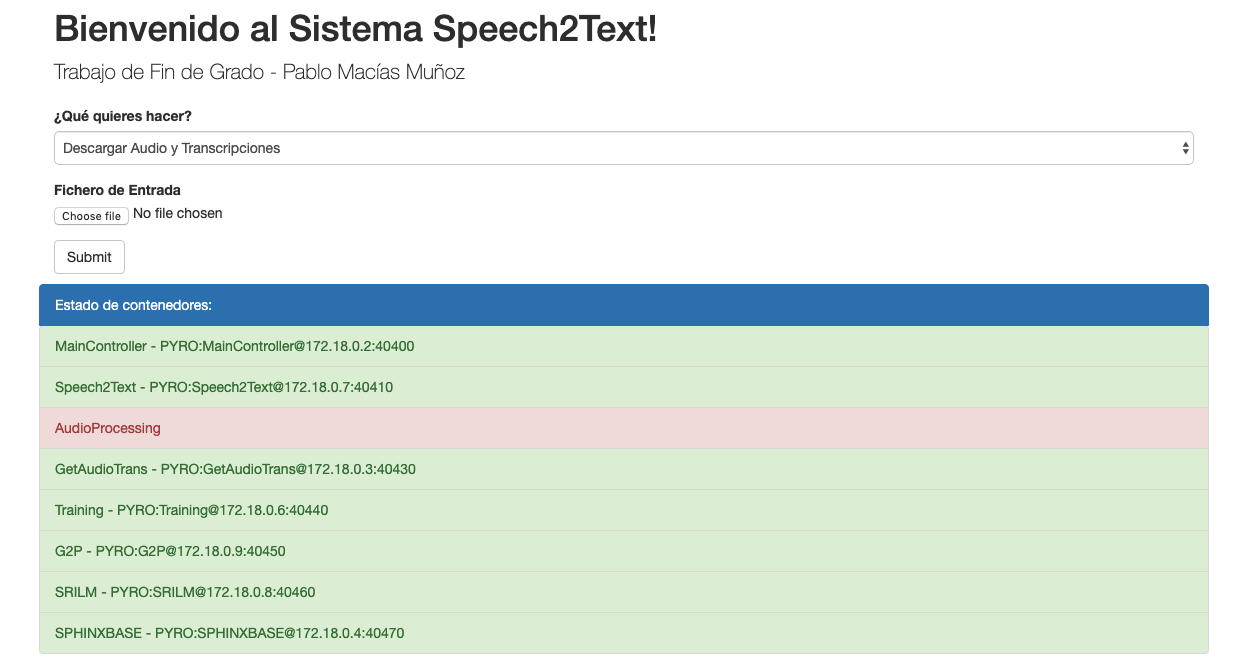
\includegraphics[width=\linewidth]{interfaz_web.png}
     \caption{Interfaz de usuario de la Aplicación Web.}
     \label{img:interfaz-web-anexo}
 \end{figure}
 
 En esta interfaz se podrá controlar el estado actual de los contenedores apareciendo en rojo si el componente está apagado, o verde si está encendido y tiene conexión con el controlador principal. Este listado se actualiza en tiempo real.
 
 También se podrá acceder a la herramienta gestora de contenedores Portainer. En esta herramienta se podrán gestionar los estados de los contenedores (encender y apagar), las redes, los volúmenes, .... Algo bastante interesante y con gran utilidad es la posibilidad de ejecutar una terminal en el contenedor en ejecución a través de la interfaz web. Algunas capturas de pantalla se muestran en la \autoref{fig:exam-portainer}.
 
  \begin{figure}[H]
  \centering
  \begin{subfigure}[b]{\linewidth}
    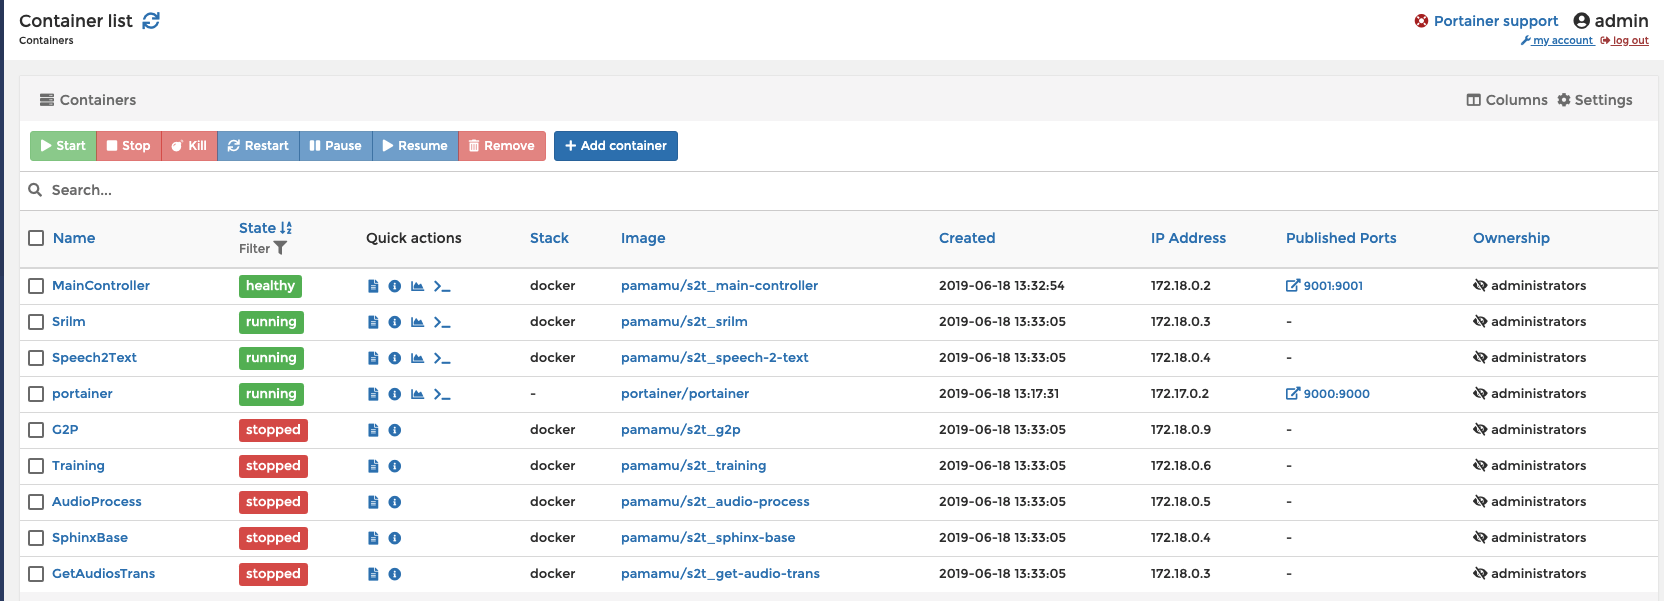
\includegraphics[width=\linewidth]{portainer-3}
    \caption{Listado de contenedores.}
  \end{subfigure}
  \begin{subfigure}[b]{0.50\linewidth}
    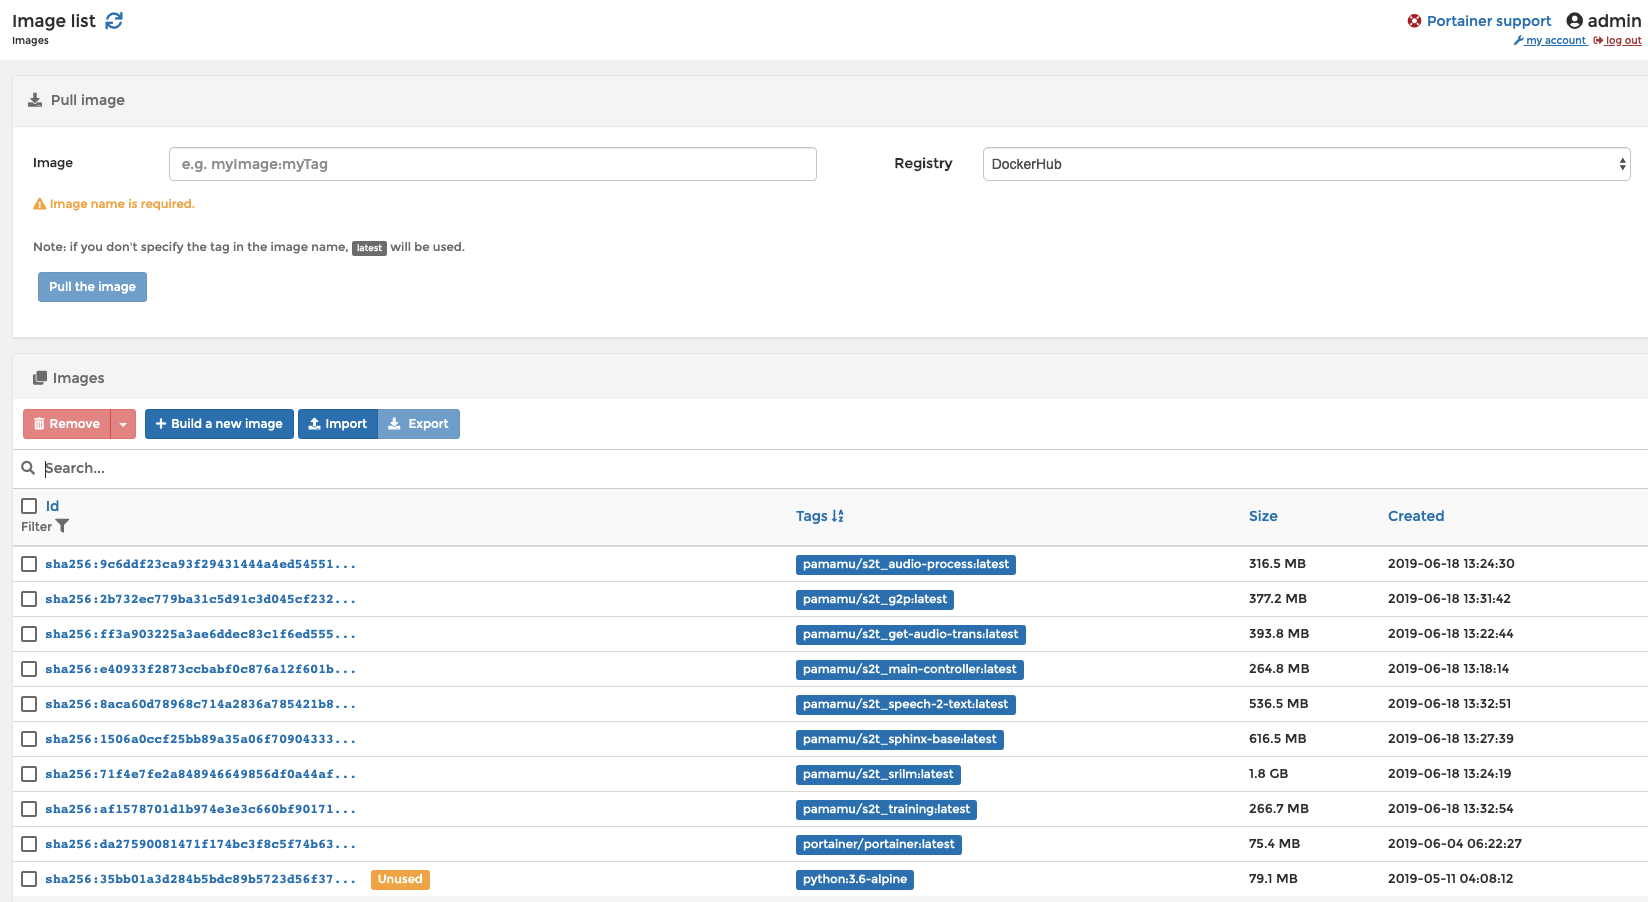
\includegraphics[width=\linewidth]{portainer-4}
    \caption{Listado de imágenes.}
  \end{subfigure}\hfill
  \begin{subfigure}[b]{0.45\linewidth}
    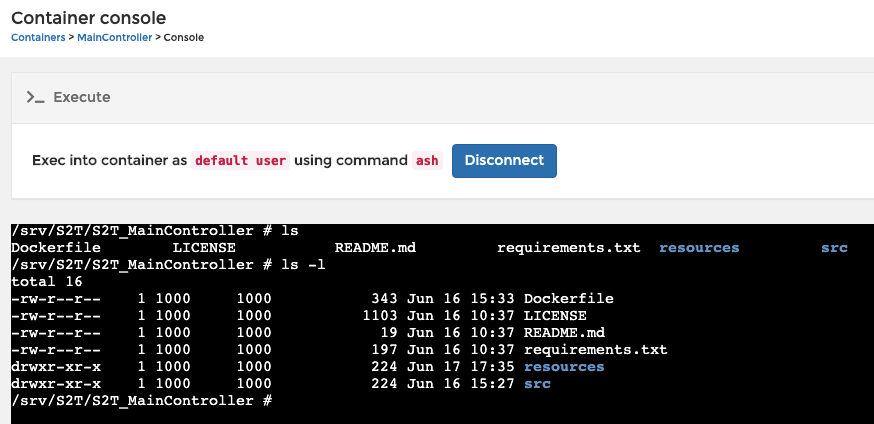
\includegraphics[width=\linewidth]{portainer-5}
    \caption{Ejecución de terminal en un contenedor.}
  \end{subfigure}
  \caption{Pantallas principales Portainer.}
  \label{fig:exam-portainer}
\end{figure}
 
 En la primera ejecución se necesitará la creación de un usuario y la configuración del \textit{endpoint} del servicio de docker (Local) como se puede observar en la \autoref{fig:conf-portainer}.
 
 \begin{figure}[H]
  \centering
  \begin{subfigure}[b]{0.40\linewidth}
    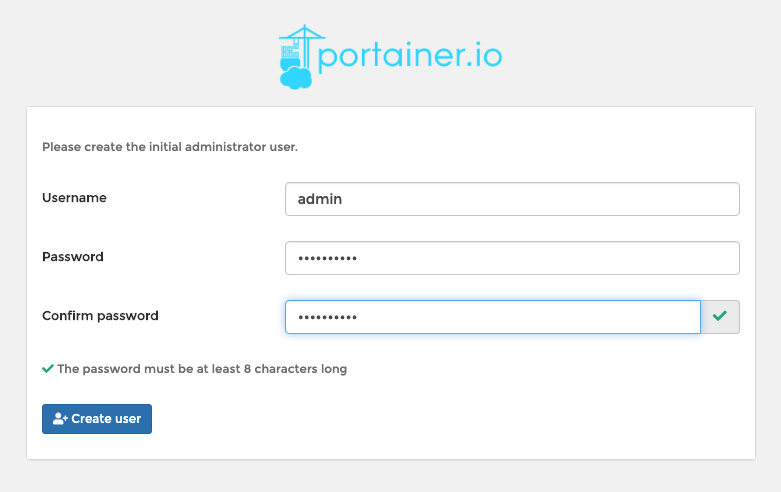
\includegraphics[width=\linewidth]{portainer-1}
    \caption{Creación de usuario}
  \end{subfigure}\hfill
  \begin{subfigure}[b]{0.45\linewidth}
    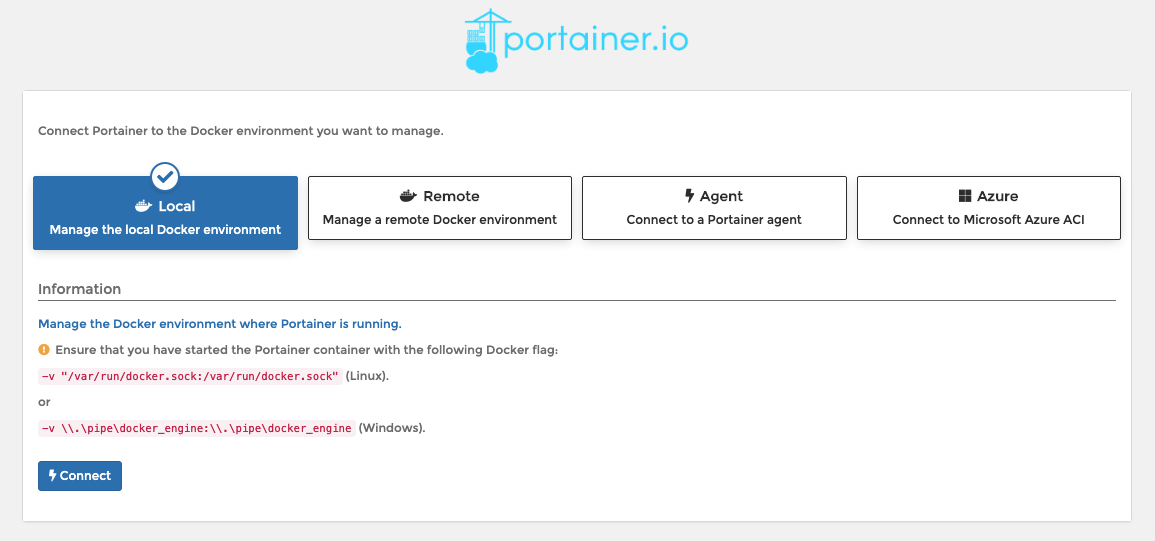
\includegraphics[width=\linewidth]{portainer-2}
    \caption{Configuración de endpoint}
  \end{subfigure}
  \caption{Configuración inicial Portainer}
  \label{fig:conf-portainer}
\end{figure}

\end{document}